%==============================================================================
%  Complexity and Noise-Resilience of Quantum Oracles for Symmetric Cryptanalysis
%
%  Build:
%     pdflatex report
%     bibtex   report
%     pdflatex report
%     pdflatex report
%
%  Every numerical value in this document is pulled from results_generated.tex,
%  which scripts/make_report_macros.py writes directly from results/data/*.json.
%  Do not hard-code results here: re-run the experiments, re-run that script,
%  and the report follows the data.
%==============================================================================
\documentclass[11pt,a4paper]{article}

\usepackage[utf8]{inputenc}
\usepackage[T1]{fontenc}
\usepackage[margin=1in]{geometry}
\usepackage{amsmath,amssymb}
\usepackage{graphicx}
\usepackage{booktabs}
\usepackage{multirow}
\usepackage{caption}
\usepackage{xcolor}
\usepackage{listings}
\usepackage[numbers,sort&compress]{natbib}
\usepackage[hidelinks]{hyperref}

\graphicspath{{../../results/figures/}}

\lstset{
  basicstyle=\ttfamily\footnotesize,
  breaklines=true,
  frame=single,
  rulecolor=\color{gray!40},
  backgroundcolor=\color{gray!5},
  columns=fullflexible,
  keepspaces=true,
}

% Numbers, tables and macros generated from the experiment records.
% Auto-generated by scripts/make_report_macros.py -- DO NOT EDIT.
% Every number in the report comes from results/data/*.json via these
% macros, so the prose cannot drift from the data.

% ---- run metadata ------------------------------------------------
\newcommand{\RunShots}{4,096}
\newcommand{\RunSeed}{20260902}
\newcommand{\RunKeyBits}{4}
\newcommand{\RunRounds}{2}
\newcommand{\RunKeySpace}{16}
\newcommand{\RunSecretKey}{\texttt{1101}}
\newcommand{\RunPairs}{1}
\newcommand{\RunSolutions}{1}
\newcommand{\RunQubits}{8}
\newcommand{\RunKstar}{3}
\newcommand{\RunQiskit}{2.5.2}
\newcommand{\RunAer}{0.17.2}
\newcommand{\RunPython}{3.13.3}

% ---- Experiment A -- ideal ---------------------------------------
\newcommand{\AbestK}{3}
\newcommand{\AbestP}{0.9613}
\newcommand{\AdeviationSci}{4.33\times10^{-15}}
\newcommand{\AoverRotation}{yes}
\newcommand{\AexactZero}{0.0625}
\newcommand{\AexactOne}{0.4727}
\newcommand{\AexactTwo}{0.9084}
\newcommand{\AexactThree}{0.9613}
\newcommand{\AexactFour}{0.5817}
\newcommand{\AexactFive}{0.1255}
\newcommand{\AexactSix}{0.0204}
\newcommand{\AuniformP}{0.0625}
\newcommand{\AmaxK}{6}
\newcommand{\Aruntime}{3.9}

% ---- Experiment B -- noisy ---------------------------------------
\newcommand{\BpOne}{10^{-3}}
\newcommand{\BpTwo}{10^{-2}}
\newcommand{\BreadoutZeroOne}{2\%}
\newcommand{\BreadoutOneZero}{4\%}
\newcommand{\Bcx}{1,404}
\newcommand{\Bdepth}{4,861}
\newcommand{\BidealP}{0.9613}
\newcommand{\BnoisyP}{0.0574}
\newcommand{\BnoisyErr}{0.0036}
\newcommand{\Btvd}{0.9039}
\newcommand{\Bentropy}{3.995}
\newcommand{\BentropyMax}{4.000}
\newcommand{\Bsigmas}{-1.4}
\newcommand{\Bsignificant}{no}
\newcommand{\Bruntime}{1087.8}

% ---- Experiment C -- mitigation ----------------------------------
\newcommand{\CidealP}{0.9613}
\newcommand{\Citerations}{3}
\newcommand{\CreducedScale}{0.03}
\newcommand{\Cruntime}{319.9}
\newcommand{\CcalibrationCircuits}{16}
\newcommand{\CReadoutRaw}{0.8408}
\newcommand{\CReadoutRawTvd}{0.1225}
\newcommand{\CReadoutFidelity}{0.8852}
\newcommand{\CReadoutCond}{1.30}
\newcommand{\CReadoutPinvP}{0.9692}
\newcommand{\CReadoutPinvTvd}{0.0143}
\newcommand{\CReadoutPinvNeg}{0.0049}
\newcommand{\CReadoutPinvValid}{no}
\newcommand{\CReadoutPinvGain}{0.1283}
\newcommand{\CReadoutClipP}{0.9644}
\newcommand{\CReadoutClipTvd}{0.0119}
\newcommand{\CReadoutClipNeg}{0.0000}
\newcommand{\CReadoutClipValid}{yes}
\newcommand{\CReadoutClipGain}{0.1236}
\newcommand{\CReadoutNnlsP}{0.9652}
\newcommand{\CReadoutNnlsTvd}{0.0127}
\newcommand{\CReadoutNnlsNeg}{0.0000}
\newcommand{\CReadoutNnlsValid}{yes}
\newcommand{\CReadoutNnlsGain}{0.1243}
\newcommand{\CReducedRaw}{0.6343}
\newcommand{\CReducedRawTvd}{0.3270}
\newcommand{\CReducedFidelity}{0.8849}
\newcommand{\CReducedCond}{1.30}
\newcommand{\CReducedPinvP}{0.7325}
\newcommand{\CReducedPinvTvd}{0.2288}
\newcommand{\CReducedPinvNeg}{0.0000}
\newcommand{\CReducedPinvValid}{yes}
\newcommand{\CReducedPinvGain}{0.0982}
\newcommand{\CReducedClipP}{0.7325}
\newcommand{\CReducedClipTvd}{0.2288}
\newcommand{\CReducedClipNeg}{0.0000}
\newcommand{\CReducedClipValid}{yes}
\newcommand{\CReducedClipGain}{0.0982}
\newcommand{\CReducedNnlsP}{0.7325}
\newcommand{\CReducedNnlsTvd}{0.2288}
\newcommand{\CReducedNnlsNeg}{0.0000}
\newcommand{\CReducedNnlsValid}{yes}
\newcommand{\CReducedNnlsGain}{0.0982}
\newcommand{\CFullRaw}{0.0574}
\newcommand{\CFullRawTvd}{0.9039}
\newcommand{\CFullFidelity}{0.8839}
\newcommand{\CFullCond}{1.30}
\newcommand{\CFullPinvP}{0.0596}
\newcommand{\CFullPinvTvd}{0.9017}
\newcommand{\CFullPinvNeg}{0.0000}
\newcommand{\CFullPinvValid}{yes}
\newcommand{\CFullPinvGain}{0.0022}
\newcommand{\CFullClipP}{0.0596}
\newcommand{\CFullClipTvd}{0.9017}
\newcommand{\CFullClipNeg}{0.0000}
\newcommand{\CFullClipValid}{yes}
\newcommand{\CFullClipGain}{0.0022}
\newcommand{\CFullNnlsP}{0.0596}
\newcommand{\CFullNnlsTvd}{0.9017}
\newcommand{\CFullNnlsNeg}{0.0000}
\newcommand{\CFullNnlsValid}{yes}
\newcommand{\CFullNnlsGain}{0.0022}

% ---- Experiment D -- threshold -----------------------------------
\newcommand{\Dcx}{1,404}
\newcommand{\Ddepth}{4,861}
\newcommand{\Druntime}{1214.6}
\newcommand{\DmaxWorkingPtwo}{3.0\times10^{-3}}
\newcommand{\DuniformP}{0.0625}
\newcommand{\DfirstFailingPtwo}{10^{-2}}
\newcommand{\DmaxWorkingP}{0.1282}

% ---- Experiment E -- resources -----------------------------------
\newcommand{\Eruntime}{4.7}
\newcommand{\EminKeyBits}{4}
\newcommand{\EmaxKeyBits}{8}
\newcommand{\EmaxCx}{33,360}
\newcommand{\EmaxDepth}{96,604}
\newcommand{\EmaxQubits}{20}
\newcommand{\EmaxSpeedup}{21.3}
\newcommand{\EmaxDensityGB}{16384.0}
\newcommand{\EmaxStatevectorMB}{16.000}
\newcommand{\EminCx}{1,404}


% amsmath provides no Dirac notation, and physics/braket are not present in
% every TeX distribution, so define what we need here.
\newcommand{\ket}[1]{\left|#1\right\rangle}
\newcommand{\bra}[1]{\left\langle#1\right|}

\newcommand{\Ek}{E_K}
\newcommand{\bigO}[1]{\mathcal{O}\!\left(#1\right)}

\title{\bfseries Complexity and Noise-Resilience of Quantum Oracles\\
       for Symmetric Cryptanalysis\\[0.4em]
       \large A Reproducible Study of Grover Key Search on a 4-bit SPN\\
       under Simulated NISQ Noise}
\author{Luke\\ \small\texttt{luke@ai4group.com.au}}
\date{\today}

\begin{document}
\maketitle

\begin{abstract}
\noindent
We construct and validate a reversible quantum oracle for known-plaintext key
search against a toy 4-bit substitution--permutation network, apply Grover's
algorithm~\citep{grover1996} to recover the key, and quantify how the attack
degrades under simulated NISQ noise~\citep{preskill2018}. The oracle evaluates
the cipher on the key register in superposition and compares the result against
known ciphertexts, so at no point does it presuppose the secret key. Its
correctness is established exhaustively: the encryption circuit's exact unitary
is verified against an independent classical reference for every key and
plaintext, and the oracle is shown to restore its data registers completely,
which is the property on which Grover interference depends.

Ideal simulation reproduces the closed-form amplification curve
$\sin^2\!\big((2k{+}1)\theta\big)$ to within $\AdeviationSci$, including the
over-rotation decline beyond the optimal iteration count. Under depolarizing
and readout noise at contemporary hardware rates ($p_2 = \BpTwo$), the
$\Bcx$-CX circuit is driven to an output entropy of $\Bentropy$ bits against a
maximum of $\BentropyMax$: amplification is not merely degraded but absent. We
then apply classical readout-error mitigation by assignment-matrix inversion
and obtain the paper's central result, a \emph{boundary}. When measurement
error is the only channel, mitigation restores the success probability from
$\CReadoutRaw$ to $\CReadoutNnlsP$ against an ideal $\CidealP$; when gate error
is also present it moves the result only from $\CFullRaw$ to $\CFullNnlsP$,
both of which are random guessing. We further show that unconstrained
pseudo-inverse mitigation returns a negative probability mass of
$\CReadoutPinvNeg$ and \emph{overshoots} the ideal value, whereas a
non-negative least-squares formulation remains physical. A noise sweep places
the largest two-qubit error rate still permitting recovery at
$\DmaxWorkingPtwo$, one to two orders of magnitude below current devices, and a
resource scan shows the quadratic query saving being purchased with circuits
growing from $\EminCx$ to $\EmaxCx$ CX gates between $\EminKeyBits$- and
$\EmaxKeyBits$-bit keys. All code, data and figures are released for
reproduction.
\end{abstract}

\tableofcontents
\bigskip

%==============================================================================
\section{Introduction}
%==============================================================================

Grover's algorithm provides a quadratic speedup for unstructured
search~\citep{grover1996} and this bound is known to be
optimal~\citep{bennett1997,zalka1999}. Applied to symmetric cryptography, it
reduces the cost of exhaustive key search from $\bigO{2^n}$ to $\bigO{2^{n/2}}$
oracle queries, which is the standard justification for doubling symmetric key
lengths in post-quantum guidance~\citep{nistir8105,bernstein2017}.

That query-complexity statement, however, says nothing about whether such an
attack is \emph{implementable}. Two questions sit between the asymptotic
speedup and a real threat:

\begin{enumerate}
  \item \textbf{What does one oracle query actually cost?} The oracle must
        contain a full reversible implementation of the cipher. Detailed
        resource estimates for AES~\citep{grassl2016,jaques2020} and
        SHA~\citep{amy2016} show this circuit, not the query count, dominates
        the cost.
  \item \textbf{Does amplification survive hardware noise?} Grover depends on
        coherent interference across the whole search register. Present-day
        devices are noisy~\citep{preskill2018}, and error mitigation, while
        able to extend useful computational reach~\citep{kandala2019,cai2023},
        is not error correction.
\end{enumerate}

This report addresses both questions on a deliberately small but genuine
instance. We use a 4-bit substitution--permutation network built from the
published PRESENT S-box~\citep{bogdanov2007} in the structure of the classical
SPN teaching model~\citep{heys2002}. The key space is tiny, which is precisely
what makes exhaustive verification of every claim affordable: we check the
quantum circuit against a classical reference for \emph{all} keys and
plaintexts rather than sampling.

\subsection{Contributions}

\begin{itemize}
  \item A \textbf{non-circular} reversible key-search oracle: it evaluates
        $\Ek(P)$ in superposition and compares against known ciphertexts,
        rather than being handed the target key. It uses
        $n + 4r$ qubits and \textbf{no ancillas}.
  \item \textbf{Exhaustive correctness verification} of both the encryption
        unitary and the oracle's uncomputation, the latter being a failure mode
        that produces correct-looking phases with silently broken amplification.
  \item A measured demonstration that \textbf{a single known-plaintext pair
        does not determine the key}, reproducing at toy scale the multi-block
        requirement of the AES oracle literature~\citep{grassl2016,jaques2020},
        together with the gap between the information-theoretic bound and the
        number of pairs actually needed.
  \item \textbf{Localisation of the boundary of readout-error mitigation}: near
        complete recovery of a readout-limited signal, and no recovery
        whatsoever of a gate-error-limited one, measured under three noise
        models that differ only in gate error.
  \item A demonstration that \textbf{unconstrained inversion is unphysical} in
        practice, not just in principle, reproducing the unfolding
        pathology~\citep{nachman2020} at small scale.
  \item An explicit account of the \textbf{simulation resource trade}:
        trajectory sampling reduces noisy-simulation memory from $\bigO{4^n}$ to
        $\bigO{2^n}$, converting a memory barrier into a runtime cost.
\end{itemize}

%==============================================================================
\section{Background}
%==============================================================================

\subsection{Symmetric key search as an oracle problem}

In a known-plaintext attack the adversary holds pairs $(P_i, C_i)$ with
$C_i = \Ek[K^\ast](P_i)$ for an unknown key $K^\ast$, and seeks
\begin{equation}
  K^\ast \in \Big\{\, K \in \{0,1\}^n \;:\; \Ek(P_i) = C_i \ \ \forall i \,\Big\}.
\end{equation}
Classically this requires up to $2^n$ trial encryptions. The corresponding
Boolean predicate
\begin{equation}
  f(K) = \begin{cases}
    1 & \text{if } \Ek(P_i) = C_i \text{ for every } i,\\
    0 & \text{otherwise,}
  \end{cases}
  \label{eq:predicate}
\end{equation}
is exactly the marking function Grover's algorithm requires. Note that
Eq.~\eqref{eq:predicate} references only $(P_i, C_i)$ --- the data an attacker
possesses --- and never $K^\ast$.

\subsection{Reversibility}

Quantum evolution is unitary, hence reversible, so an irreversible classical
function cannot be inserted into a circuit directly. The standard remedy embeds
it as
\begin{equation}
  U_f \ket{x}\ket{y} = \ket{x}\ket{y \oplus f(x)},
\end{equation}
a construction resting on Bennett's demonstration that any computation can be
made logically reversible~\citep{bennett1973}, itself motivated by Landauer's
result that irreversible bit erasure carries an unavoidable thermodynamic
cost~\citep{landauer1961}. For a \emph{phase} oracle we instead want
\begin{equation}
  O_f \ket{K} = (-1)^{f(K)} \ket{K},
  \label{eq:phase-oracle}
\end{equation}
which Section~\ref{sec:oracle} realises without any ancilla register.

\subsection{Grover search}

Beginning from the uniform superposition
$\ket{s} = N^{-1/2}\sum_{x=0}^{N-1}\ket{x}$ with $N = 2^n$, Grover alternates
the phase oracle~\eqref{eq:phase-oracle} with the diffusion operator
$D = 2\ket{s}\!\bra{s} - I$. With $M$ marked states and
$\theta = \arcsin\sqrt{M/N}$, the probability of measuring a marked state after
$k$ iterations is
\begin{equation}
  P(k) = \sin^2\!\big((2k+1)\,\theta\big),
  \label{eq:grover-prob}
\end{equation}
maximised at
\begin{equation}
  k^\ast = \left\lfloor \frac{\pi}{4}\sqrt{\frac{N}{M}} \right\rfloor .
  \label{eq:kstar}
\end{equation}
Two consequences of Eq.~\eqref{eq:grover-prob} are frequently misstated and are
measured directly in Section~\ref{sec:results-a}. First, $k^\ast$ is
\emph{not} $\sqrt{N}$; the factor $\pi/4$ and the dependence on $M$ both
matter~\citep{boyer1998}. Second, $P(k)$ is periodic, so exceeding $k^\ast$
\emph{reduces} the success probability. Amplitude amplification generalises this
to arbitrary state preparation~\citep{brassard2002}; a full derivation appears
in~\citet[Ch.~6]{nielsen2010}.

\subsection{NISQ noise and error mitigation}

Contemporary processors operate without error correction, in what
\citet{preskill2018} termed the NISQ regime. We model two channels. The
depolarizing channel replaces a state with the maximally mixed state with
probability $p$,
\begin{equation}
  \mathcal{E}_p(\rho) = (1-p)\,\rho + p\,\frac{I}{2^m},
\end{equation}
applied at rate $p_1$ to single-qubit and $p_2$ to two-qubit gates. Readout
error is an asymmetric classical bit flip at measurement time.

Error \emph{mitigation} differs fundamentally from error correction: it applies
classical post-processing to recover expectation values or distributions
without correcting any quantum state~\citep{cai2023}. Two families are
relevant. Zero-noise extrapolation runs a circuit at deliberately amplified
noise and extrapolates to the zero-noise
limit~\citep{temme2017,li2017,kandala2019}. Readout-error mitigation, which we
implement, characterises the measurement channel and inverts
it~\citep{bravyi2021,nation2021}. The distinction matters for interpreting our
results: readout mitigation addresses only the measurement step, and
Section~\ref{sec:results-c} measures the consequence.

%==============================================================================
\section{The cipher}
%==============================================================================

We use a 4-bit block SPN with an $n$-bit master key ($n = \RunKeyBits$ by
default) and $r$ rounds ($r = \RunRounds$):
\begin{equation}
  \Ek(P) \;=\; \mathrm{ARK}_{rk_r} \circ \Big( \pi \circ S \Big) \circ \cdots
                \circ \mathrm{ARK}_{rk_1} \circ \Big( \pi \circ S \Big)
                \circ \mathrm{ARK}_{rk_0}(P),
\end{equation}
giving $r$ substitution layers and $r+1$ key additions.

\paragraph{Substitution.} $S$ is the PRESENT 4-bit
S-box~\citep{bogdanov2007}, a published cryptographic primitive rather than an
ad-hoc permutation:
\[
\begin{array}{c|cccccccccccccccc}
x    & 0 & 1 & 2 & 3 & 4 & 5 & 6 & 7 & 8 & 9 & \mathrm{A} & \mathrm{B} & \mathrm{C} & \mathrm{D} & \mathrm{E} & \mathrm{F}\\
\hline
S[x] & \mathrm{C} & 5 & 6 & \mathrm{B} & 9 & 0 & \mathrm{A} & \mathrm{D} & 3 & \mathrm{E} & \mathrm{F} & 8 & 4 & 7 & 1 & 2
\end{array}
\]

\paragraph{Permutation.} $\pi$ is the fixed bit permutation
$(0 \mapsto 1,\, 1 \mapsto 3,\, 2 \mapsto 0,\, 3 \mapsto 2)$, deliberately not a
rotation so that diffusion is not trivially self-similar with the key schedule.

\paragraph{Key schedule.} Round key $rk_j = \mathrm{rotl}(K, j) \wedge \mathtt{0xF}$.
This choice is made for a quantum-implementation reason: a rotation is
\emph{free} on a quantum register, since XOR-ing $\mathrm{rotl}(K,j)$ into the
data register only changes \emph{which key qubit acts as the CNOT control}. A
schedule involving substitutions would have to be computed and uncomputed
inside every oracle call.

The classical implementation (\texttt{spn.py}) depends on nothing beyond the
Python standard library and shares no code with the quantum implementation.
This independence is deliberate: it makes the equivalence check of
Section~\ref{sec:validation} a genuine cross-check rather than a tautology.

%==============================================================================
\section{The reversible oracle}
\label{sec:oracle}
%==============================================================================

\subsection{Construction}

The oracle is built as \textbf{compute\,--\,phase\,--\,uncompute}. Let $U_E$ be
the reversible, key-controlled encryption acting in place on a 4-qubit data
register, and let there be $r$ known pairs, each with its own data register
initialised to $\ket{P_i}$.

\begin{enumerate}
  \item \textbf{Compute.} Apply $U_E$ to each data register, with the key
        register providing CNOT controls only:
        \[
          \sum_K \ket{K}\ket{P_1 \cdots P_r}
          \;\longmapsto\;
          \sum_K \ket{K}\ket{\Ek(P_1) \cdots \Ek(P_r)}.
        \]
  \item \textbf{Phase.} Conjugate a multi-controlled $Z$ over all $4r$ data
        qubits by an $X$-mask encoding the concatenated target ciphertext, so a
        $-1$ phase is applied exactly when every register holds its target.
  \item \textbf{Uncompute.} Apply $U_E^\dagger$ to each data register.
\end{enumerate}

Because the phase is diagonal it commutes through step 3, giving
\begin{equation}
  \sum_K \ket{K}\ket{P_1 \cdots P_r}
  \;\longmapsto\;
  \sum_K (-1)^{f(K)} \ket{K}\ket{P_1 \cdots P_r},
\end{equation}
with the data registers restored and therefore factored out.

\subsection{Why uncomputation is decisive}

This is the construction's most important subtlety. Omitting step 3 still
yields an oracle that marks the correct states with the correct phases. But the
key register is then entangled with the data registers, and that residual
which-path information destroys the interference on which the diffusion
operator relies: amplification silently fails to accumulate. It is a defect
that inspects as correct and behaves as wrong, which is why
Section~\ref{sec:validation} tests for it explicitly, asserting that the
entire probability mass returns to the restored-plaintext subspace.

\subsection{Ancilla-free by construction}

The oracle uses $n + 4r$ qubits and no ancillas. Two structural facts make this
possible. Every cipher layer --- key XOR, S-box, bit permutation --- is
individually a bijection on 4 bits and therefore acts in place. And the $r$
separate 4-bit equality tests are fused into a \emph{single} $4r$-qubit AND
condition, rather than computing $r$ flag qubits and combining them; flags would
themselves require uncomputation.

\subsection{One plaintext pair is not enough}
\label{sec:pairs}

For a 4-bit block, $K \mapsto \Ek(P)$ is not injective, so a single known pair
generally leaves several consistent keys. Exhaustive measurement over the whole
key space at $r = 2$ gives Table~\ref{tab:pairs}.

\begin{table}[htbp]
  \centering
  \caption{Consistent keys versus number of known plaintext/ciphertext pairs,
           measured exhaustively over all $16$ keys ($n=4$, $r=2$).}
  \label{tab:pairs}
  \begin{tabular}{cccc}
    \toprule
    Known pairs & Worst-case $M$ & Mean $M$ & Keys uniquely determined \\
    \midrule
    1 & 3 & 1.88 & 8 / 16 \\
    2 & 2 & 1.25 & 12 / 16 \\
    3 & \textbf{1} & 1.00 & \textbf{16 / 16} \\
    \bottomrule
  \end{tabular}
\end{table}

This is not an artefact of the toy scale. It is the same counting argument that
requires quantum key-search oracles against AES-128 to encrypt several
plaintext blocks~\citep{grassl2016,jaques2020}. Measured across key widths, the
information-theoretic estimate $\lceil n/4 \rceil + 1$ is a \emph{lower} bound:
at $n=4$ between $1$ and $3$ pairs are needed depending on the key, at $n=6$
exactly $3$, and at $n=8$ between $3$ and $4$. The implementation therefore
grows the pair count until classical brute force confirms $M = 1$, and reports
the number used. Each additional pair costs a further 4-qubit register and two
more encryption circuits per oracle call, making this the dominant cost driver.

%==============================================================================
\section{Method}
%==============================================================================

\subsection{Simulation and the memory--time trade}
\label{sec:memory}

Simulation uses Qiskit~\citep{qiskit2024} with the Aer backend. One
configuration choice dominates feasibility. Noisy simulation admits two
representations, and their scaling differs qualitatively:

\begin{table}[htbp]
  \centering
  \caption{Memory required for noisy simulation. Aer's \texttt{automatic} method
           may select density-matrix simulation once a noise model is attached.}
  \label{tab:memory}
  \begin{tabular}{lrrrr}
    \toprule
    Method & Scaling & 8 qubits & 16 qubits & 20 qubits \\
    \midrule
    Density matrix           & $\bigO{4^n}$ & 1\,MB & 68\,GB & 17.6\,TB \\
    Statevector trajectories & $\bigO{2^n}$ & 4\,KB & 1\,MB  & 16\,MB \\
    \bottomrule
  \end{tabular}
\end{table}

We therefore pin the simulation method to \texttt{statevector}, which makes Aer
use stochastic quantum trajectories: one pure state per shot, sampling a Kraus
operator at each noisy gate, with the shot average converging to the same
density-matrix result. This reduces memory from $\bigO{4^n}$ to $\bigO{2^n}$ at
the cost of runtime scaling as
\begin{equation}
  T \;\propto\; \text{shots} \times \text{gates} \times 2^{n_{\mathrm{qubits}}} .
  \label{eq:runtime}
\end{equation}
It is worth stating precisely what is and is not saved here. Shot-based sampling
does not avoid storing a statevector --- Aer maintains one either way. What
trajectory sampling avoids is the \emph{density matrix}. The saving is
$4^n \to 2^n$, and it is what allows this study to run on a single laptop.

\paragraph{A transpilation prerequisite.} A noise model binds errors to
\emph{named basis gates}. A circuit still containing composite instructions
(a generic \texttt{UnitaryGate}, a multi-controlled $Z$, a \texttt{swap})
contains no \texttt{cx} or \texttt{sx} for the model to attach to, and would
execute essentially noise-free while appearing to be noisy --- with no error
raised anywhere. Every execution path therefore transpiles to the IBM-native
basis $\{\texttt{id}, \texttt{rz}, \texttt{sx}, \texttt{x}, \texttt{cx}\}$
first. The S-box is synthesised from its permutation matrix by quantum Shannon
decomposition~\citep{shende2006}. \texttt{rz} is left noiseless: on transmon
hardware a $Z$ rotation is a virtual frame change of zero duration, applied by
shifting the phase of subsequent drive pulses rather than by playing a
pulse~\citep{mckay2017}, and IBM's backend properties report no gate error for
it. Section~\ref{sec:limitations} records the sense in which this is an
idealisation.

\subsection{Noise parameters}

Single-qubit depolarizing rate $p_1 = \BpOne$, two-qubit rate
$p_2 = \BpTwo$, and asymmetric readout error with
$P(1\,|\,0) = \BreadoutZeroOne$ and $P(0\,|\,1) = \BreadoutOneZero$. The
order-of-magnitude gap between $p_1$ and $p_2$, and the readout asymmetry
(energy relaxation makes $1 \to 0$ more likely), both follow measured
superconducting-device behaviour.

\subsection{Readout-error mitigation}

Measured and true distributions are related through the assignment matrix,
\begin{equation}
  y = A x, \qquad A_{ij} = P(\text{observe } i \mid \text{prepared } j),
\end{equation}
characterised by $2^{n}$ calibration circuits over the measured qubits. Only
the key register is measured, which keeps calibration at
$\CcalibrationCircuits$ circuits rather than $2^{n+4r}$. Calibration circuits
are shallow, so $A$ captures the measurement channel rather than a mixture of
gate and readout effects.

We implement three inversions of $y = Ax$:
\begin{description}
  \item[\texttt{pinv}] the Moore--Penrose pseudo-inverse. Unbiased, but $A^{-1}$
    is not a stochastic matrix, so the result may leave the probability
    simplex~\citep{nachman2020}.
  \item[\texttt{clip}] \texttt{pinv} followed by clipping and renormalisation:
    cheap, but the clip biases the estimate.
  \item[\texttt{nnls}] $\min_x \|Ax - y\|_2$ subject to $x \ge 0$, then
    renormalised. Always a valid distribution, which is why it is our default.
    Two caveats, so the attribution is not overclaimed. This is not the
    mechanism used by M3~\citep{nation2021}, which is matrix-free -- never
    forming $A$ or its inverse -- and solves within the subspace spanned by the
    observed bitstrings; M3 shares the goal of avoiding exponential calibration,
    not the method. And \citet{nachman2020}, cited above against \texttt{pinv},
    in fact advocate iterative Bayesian unfolding over both matrix inversion
    \emph{and} least squares. We retain NNLS because it is exactly solvable and
    sufficient to establish the readout-versus-gate boundary measured in
    Section~\ref{sec:results-c}, not because it is optimal.
\end{description}
We also report $\mathrm{cond}(A)$, the amplification factor for statistical
noise under inversion --- the reason mitigation is not free.

\subsection{Experimental design}

\begin{description}
  \item[A --- Ideal.] Sweep $k$ with no noise; compare against
    Eq.~\eqref{eq:grover-prob}. Establishes oracle correctness and the
    over-rotation effect.
  \item[B --- Noisy.] Repeat under depolarizing and readout noise.
  \item[C --- Mitigation.] Apply all three inversions under \emph{three} noise
    models that hold readout error fixed and vary only gate error:
    readout-only, reduced gate error ($\times\CreducedScale$), and full gate
    error. Any difference between them is therefore attributable to gate noise.
    Running only the first would overstate the technique; only the last would
    understate it.
  \item[D --- Threshold.] Scale all error rates and locate where recovery fails,
    defined operationally as the correct key ceasing to be the single most
    likely outcome.
  \item[E --- Resources.] Transpiled cost and query complexity versus key
    width. Circuits here are transpiled but \emph{not} simulated: by
    Eq.~\eqref{eq:runtime} simulating the largest is infeasible, whereas exact
    resource counts cost seconds.
\end{description}

All runs use $\RunShots$ shots and seed $\RunSeed$
(Qiskit~\RunQiskit, Aer~\RunAer, Python~\RunPython). Every reported probability
carries a binomial standard error, and comparisons against the random-guessing
baseline require a two-sigma margin before an advantage is claimed.

\subsection{Validation}
\label{sec:validation}

Two exhaustive checks underpin every downstream result.

\paragraph{The circuit is the cipher.} For every key and every plaintext, across
five configurations, the \emph{exact unitary} of the encryption circuit is
compared against the independent classical reference:
\begin{equation}
  U_E \ket{K}\ket{X} = \ket{K}\ket{\Ek(X)}
  \qquad \forall K, X .
\end{equation}
This tests the circuit itself, not a sampled outcome.

\paragraph{The oracle uncomputes.} The oracle is checked to apply $-1$ to
exactly the marked keys and $+1$ elsewhere, \emph{and} to return the full
probability mass to the restored-plaintext subspace,
\begin{equation}
  \sum_{K} \big| \langle K, P_1\cdots P_r | O_f | \psi \rangle \big|^2 = 1 ,
\end{equation}
which is the assertion that catches incomplete uncomputation.

The oracle is additionally verified to be an involution ($O_f^2 = I$), and the
mitigation code is checked against an analytically constructed assignment
matrix so that recovery is verified \emph{exactly} rather than merely shown to
improve.

%==============================================================================
\section{Results}
%==============================================================================

\subsection{Experiment A: the implementation is exact}
\label{sec:results-a}

For the instance $n=\RunKeyBits$, $r=\RunRounds$, secret key $\RunSecretKey$
with $\RunPairs$ known pair and $M = \RunSolutions$, Eq.~\eqref{eq:kstar} gives
$k^\ast = \RunKstar$. Simulation yields a peak success probability of
$\AbestP$ at $k = \AbestK$, and agrees with Eq.~\eqref{eq:grover-prob} to a
maximum deviation of $\AdeviationSci$ (Figure~\ref{fig:amplification}).

That deviation is at the level of floating-point rounding. The implementation is
not approximately Grover; within double precision it is Grover. This is the
result that licenses interpreting everything downstream as a statement about
noise rather than about a bug.

Two features of Eq.~\eqref{eq:grover-prob} are visible directly. The peak is
$\AbestP$, not unity: with $N = \RunKeySpace$ and $M = 1$, $(2k+1)\theta$ never
lands exactly on $\pi/2$ for integer $k$, so certainty is unreachable. And
over-rotation is confirmed (\AoverRotation): success falls from $\AexactThree$
at $k = 3$ to $\AexactFour$ at $k = 4$, discarding roughly a third of the
success probability through one extra iteration.

\begin{figure}[htbp]
  \centering
  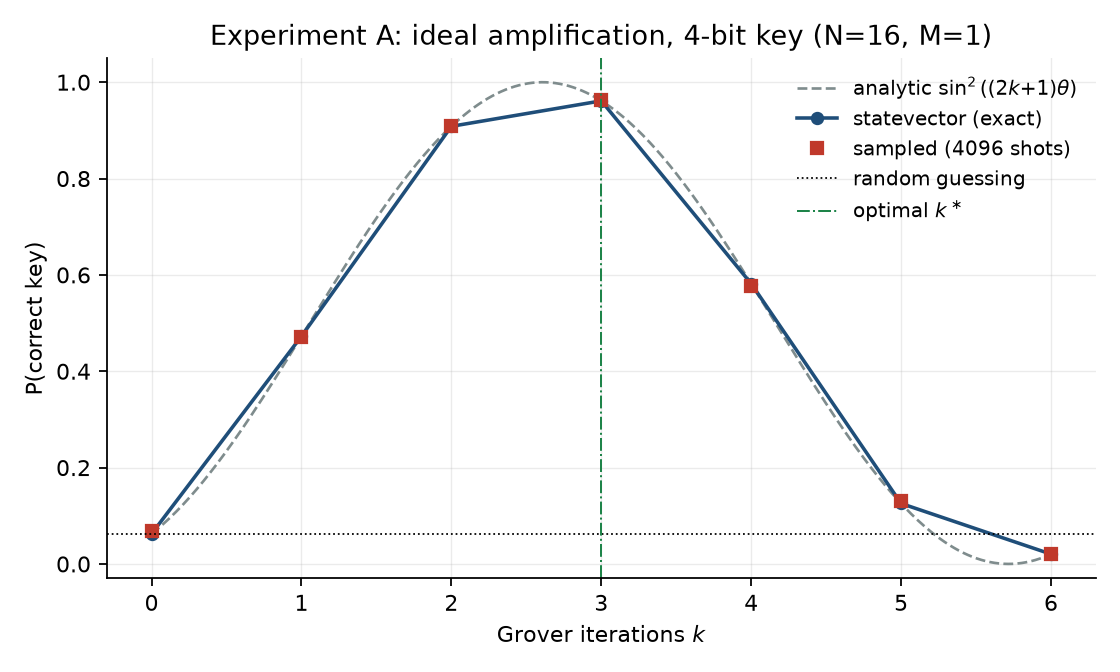
\includegraphics[width=0.86\textwidth]{fig1_amplification.png}
  \caption{Experiment A. Exact statevector probability (circles) and sampled
    result (squares) against the closed form $\sin^2((2k{+}1)\theta)$ (dashed).
    The decline beyond $k^\ast$ is the over-rotation predicted by
    Eq.~\eqref{eq:grover-prob}, not a numerical artefact.}
  \label{fig:amplification}
\end{figure}

\subsection{Experiment B: contemporary error rates destroy the attack}

At $p_1 = \BpOne$ and $p_2 = \BpTwo$ the transpiled search circuit contains
$\Bcx$ CX gates at depth $\Bdepth$. Table~\ref{tab:b} and
Figure~\ref{fig:noise} show the outcome.

\begin{table}[htbp]
  \centering
  \caption{Experiment B. Ideal versus noisy success probability across the
           iteration sweep; $k^\ast$ in bold. Entropy is in bits, against a
           uniform maximum of $\BentropyMax$.}
  \label{tab:b}
  % Auto-generated by scripts/make_report_macros.py -- DO NOT EDIT.
\begin{tabular}{rrrrrrr}
\toprule
$k$ & CX & Depth & Ideal $P$ & Noisy $P$ & TVD & Entropy \\
\midrule
0 & 0 & 4 & 0.0625 & 0.0593 & 0.026 & 3.997 \\
1 & 468 & 1,623 & 0.4727 & 0.0647 & 0.408 & 3.996 \\
2 & 936 & 3,242 & 0.9084 & 0.0583 & 0.850 & 3.996 \\
\bfseries 3 & \bfseries 1,404 & \bfseries 4,861 & \bfseries 0.9613 & \bfseries 0.0574 & \bfseries 0.904 & \bfseries 3.995 \\
4 & 1,872 & 6,480 & 0.5817 & 0.0618 & 0.520 & 3.997 \\
5 & 2,340 & 8,099 & 0.1255 & 0.0557 & 0.073 & 3.996 \\
6 & 2,808 & 9,718 & 0.0204 & 0.0623 & 0.056 & 3.996 \\
\bottomrule
\end{tabular}

\end{table}

\begin{figure}[htbp]
  \centering
  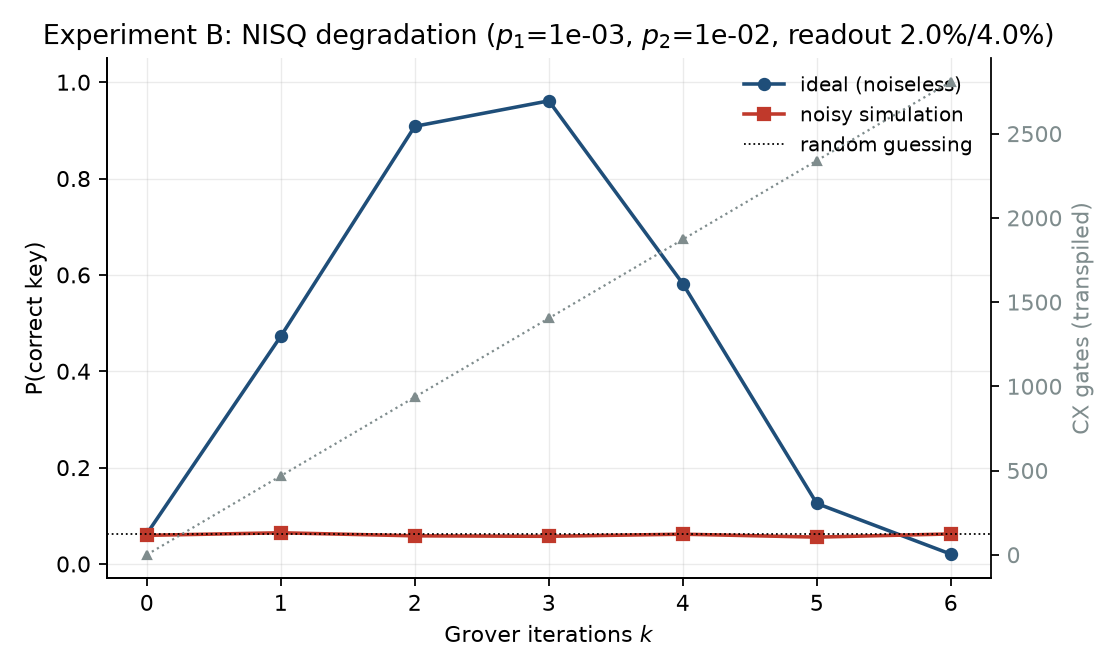
\includegraphics[width=0.86\textwidth]{fig2_noise_degradation.png}
  \caption{Experiment B. The noisy curve is flat at $1/N$ irrespective of
    iteration count: amplification does not occur at all. The dotted trace shows
    the transpiled CX count growing linearly with $k$.}
  \label{fig:noise}
\end{figure}

At $k^\ast$ the noisy success probability is
$\BnoisyP \pm \BnoisyErr$ against an ideal $\BidealP$, with
$\mathrm{TVD} = \Btvd$ and an output entropy of $\Bentropy$ bits against a
maximum of $\BentropyMax$. The output is statistically indistinguishable from
uniform, and the measured advantage over random guessing is $\Bsigmas$ standard
errors (significant: \Bsignificant).

The correct reading is stronger than ``degraded''. The noisy curve does not
track a reduced version of the ideal curve; it is flat, at the random-guessing
level, for every iteration count. Amplification is absent rather than
diminished. This is consistent with the conclusion of \citet{jaques2020} that
Grover-based key search lies far beyond near-term hardware, and we report it
without tuning the noise down to obtain a more encouraging figure.

\subsection{Experiment C: the boundary of readout mitigation}
\label{sec:results-c}

This is the report's central result. Table~\ref{tab:c} gives all three noise
models and all three inversions; Figure~\ref{fig:mitigation} shows the
distributions.

\begin{table}[htbp]
  \centering
  \caption{Experiment C. Readout error is held fixed at
    $P(1|0)=\BreadoutZeroOne$, $P(0|1)=\BreadoutOneZero$ in all three
    scenarios; only gate error varies. Ideal $P = \CidealP$. ``Valid'' means the
    result is a probability distribution.}
  \label{tab:c}
  \small
  \begin{tabular}{llrrrl}
    \toprule
    Scenario & Method & $P(\text{key})$ & TVD & Neg.\ mass & Valid \\
    \midrule
    \multirow{4}{*}{Readout only}
      & raw             & \CReadoutRaw      & \CReadoutRawTvd   & ---              & yes \\
      & \texttt{pinv}   & \CReadoutPinvP    & \CReadoutPinvTvd  & \CReadoutPinvNeg & \CReadoutPinvValid \\
      & \texttt{clip}   & \CReadoutClipP    & \CReadoutClipTvd  & \CReadoutClipNeg & \CReadoutClipValid \\
      & \texttt{nnls}   & \CReadoutNnlsP    & \CReadoutNnlsTvd  & \CReadoutNnlsNeg & \CReadoutNnlsValid \\
    \midrule
    \multirow{4}{*}{$+$ reduced gate ($\times\CreducedScale$)}
      & raw             & \CReducedRaw      & \CReducedRawTvd   & ---              & yes \\
      & \texttt{pinv}   & \CReducedPinvP    & \CReducedPinvTvd  & \CReducedPinvNeg & \CReducedPinvValid \\
      & \texttt{clip}   & \CReducedClipP    & \CReducedClipTvd  & \CReducedClipNeg & \CReducedClipValid \\
      & \texttt{nnls}   & \CReducedNnlsP    & \CReducedNnlsTvd  & \CReducedNnlsNeg & \CReducedNnlsValid \\
    \midrule
    \multirow{4}{*}{$+$ full gate error}
      & raw             & \CFullRaw         & \CFullRawTvd      & ---              & yes \\
      & \texttt{pinv}   & \CFullPinvP       & \CFullPinvTvd     & \CFullPinvNeg    & \CFullPinvValid \\
      & \texttt{clip}   & \CFullClipP       & \CFullClipTvd     & \CFullClipNeg    & \CFullClipValid \\
      & \texttt{nnls}   & \CFullNnlsP       & \CFullNnlsTvd     & \CFullNnlsNeg    & \CFullNnlsValid \\
    \bottomrule
  \end{tabular}
\end{table}

\begin{figure}[htbp]
  \centering
  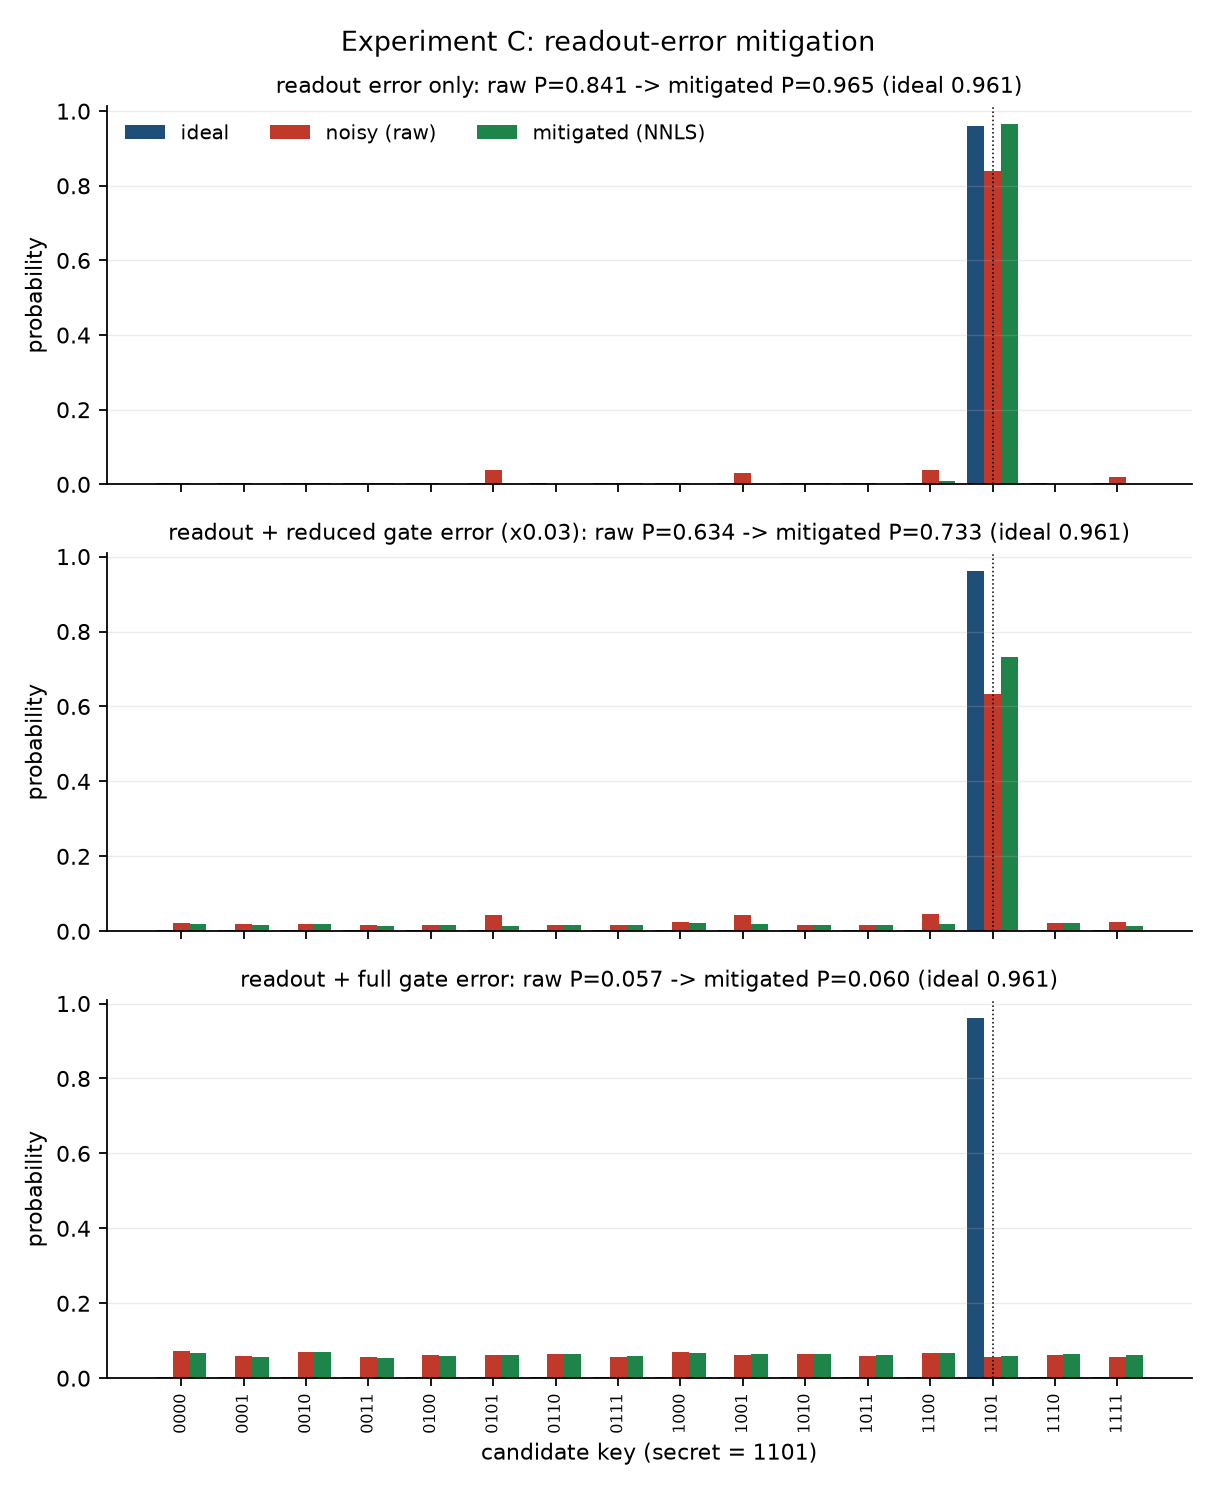
\includegraphics[width=0.94\textwidth]{fig3_mitigation.png}
  \caption{Experiment C. Per-key distributions for the three noise models.
    Mitigation restores the peak when readout error is the only channel (top)
    and cannot restore it once gate error dominates (bottom).}
  \label{fig:mitigation}
\end{figure}

\paragraph{Readout-limited: near-complete recovery.} With measurement error as
the only channel, mitigation raises the success probability from $\CReadoutRaw$
to $\CReadoutNnlsP$ against an ideal $\CidealP$, and reduces the total
variation distance from $\CReadoutRawTvd$ to $\CReadoutNnlsTvd$. Since $A$ fully
describes the corruption, inversion recovers the ideal distribution to within
shot noise. Mean readout fidelity is $\CReadoutFidelity$ with
$\mathrm{cond}(A) = \CReadoutCond$.

\paragraph{Gate-limited: no recovery at all.} With gate error at the modelled
rate, mitigation moves the result from $\CFullRaw$ to $\CFullNnlsP$. Both are
random guessing ($1/N = \DuniformP$). Nothing is recovered, and this is the
correct outcome: readout mitigation is post-processing on a classical histogram,
and once gate error has destroyed the quantum state, the information is gone
before measurement occurs. No classical operation on the histogram can restore
it.

\paragraph{The unphysicality of unconstrained inversion.} In the readout-only
scenario, \texttt{pinv} reports $P = \CReadoutPinvP$ --- \emph{higher} than the
ideal $\CidealP$ --- while placing $\CReadoutPinvNeg$ of probability mass below
zero, so it is not a valid distribution
(valid: \CReadoutPinvValid). This is not a better answer but an unphysical
overshoot, reproducing at small scale the unfolding pathology documented by
\citet{nachman2020}. The non-negative least-squares formulation sacrifices a
little accuracy to remain inside the probability simplex, which is the correct
trade and the reason it is our default.

\begin{figure}[htbp]
  \centering
  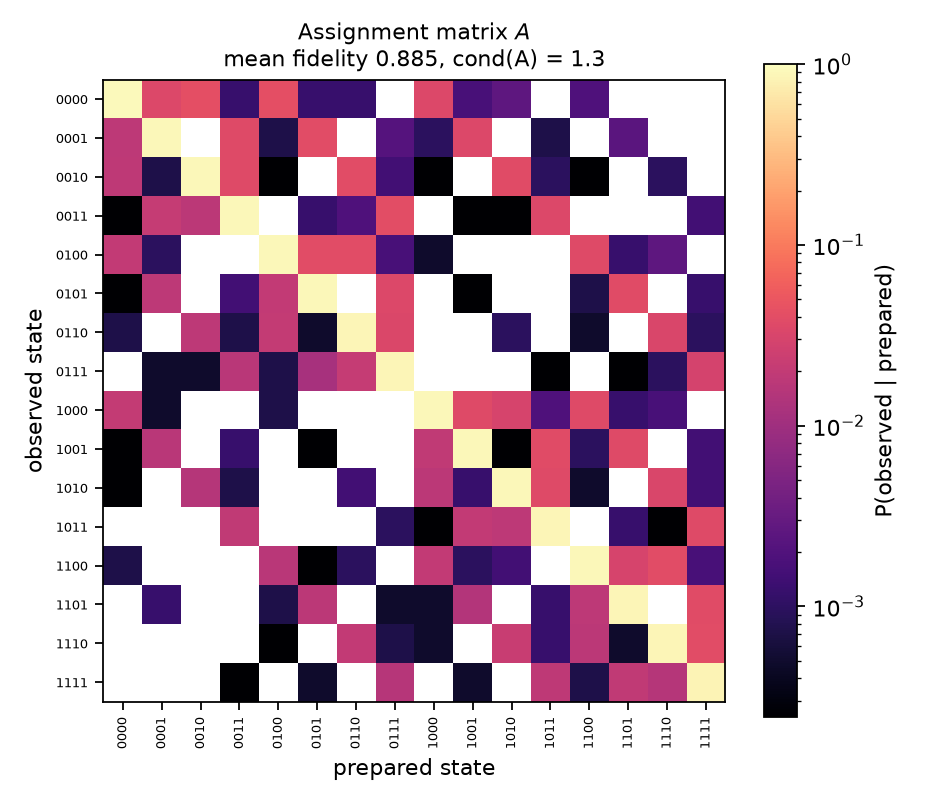
\includegraphics[width=0.62\textwidth]{fig4_assignment_matrix.png}
  \caption{The characterised assignment matrix $A$ for the measured key
    register, on a logarithmic colour scale. Off-diagonal structure is the
    readout error that mitigation inverts.}
  \label{fig:assignment}
\end{figure}

\subsection{Experiment D: how much better must hardware be?}

\begin{table}[htbp]
  \centering
  \caption{Experiment D. Success against two-qubit error rate for the
    $\Dcx$-CX, depth-$\Ddepth$ circuit. ``Checks'' is the expected number of
    classical trial encryptions if candidates are verified in descending
    probability order.}
  \label{tab:d}
  % Auto-generated by scripts/make_report_macros.py -- DO NOT EDIT.
\begin{tabular}{lrrrl}
\toprule
$p_2$ & $P(\text{key})$ & Rank of key & Checks & Key ranked first \\
\midrule
0 (ideal) & 0.9636 & 1 & 1.0 & yes \\
$10^{-5}$ & 0.9495 & 1 & 1.0 & yes \\
$3.0\times10^{-5}$ & 0.9358 & 1 & 1.0 & yes \\
$10^{-4}$ & 0.8687 & 1 & 1.0 & yes \\
$3.0\times10^{-4}$ & 0.7300 & 1 & 1.0 & yes \\
$10^{-3}$ & 0.4048 & 1 & 1.0 & yes \\
$3.0\times10^{-3}$ & 0.1282 & 1 & 1.0 & yes \\
$10^{-2}$ & 0.0574 & 13 & 13.0 & no \\
$3.0\times10^{-2}$ & 0.0530 & 14 & 14.0 & no \\
\bottomrule
\end{tabular}

\end{table}

\begin{figure}[htbp]
  \centering
  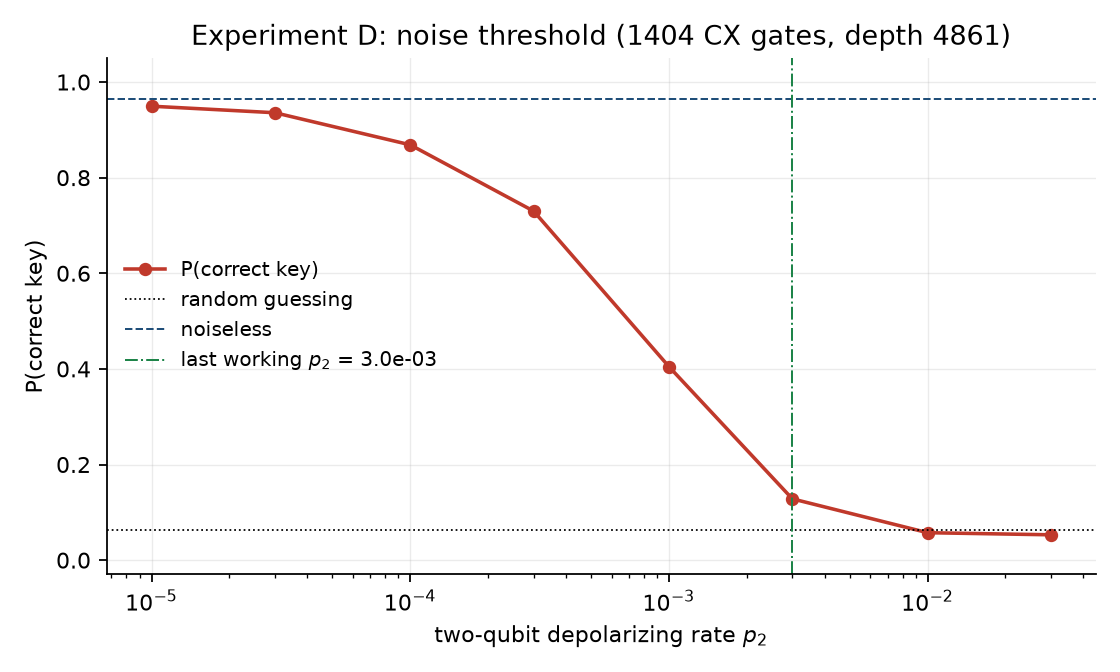
\includegraphics[width=0.86\textwidth]{fig5_noise_threshold.png}
  \caption{Experiment D. Success probability against two-qubit depolarizing
    rate. The collapse is sharp because error accumulates over $\Dcx$ CX gates.}
  \label{fig:threshold}
\end{figure}

The largest two-qubit error rate at which the correct key remains the most
likely outcome is $\DmaxWorkingPtwo$; by $\DfirstFailingPtwo$ the attack has
failed. Since contemporary superconducting two-qubit error rates sit in the
$10^{-2}$--$10^{-3}$ range, this circuit requires roughly one to two orders of
magnitude improvement.

The qualifier matters more than the number: this is a $\RunKeySpace$-key search.
The requirement is not that physical gate fidelities improve somewhat, but that
cryptographically relevant instances demand error
correction~\citep{gidney2021,acharya2024} rather than better physical gates
alone.

\subsection{Experiment E: the speedup is in queries, and queries are not free}

\begin{table}[htbp]
  \centering
  \caption{Experiment E. Transpiled resources and query complexity against key
    width. Circuits are transpiled but not simulated. ``Speedup'' is
    $2^n / k^\ast$, the query-count ratio against classical exhaustive search.}
  \label{tab:e}
  % Auto-generated by scripts/make_report_macros.py -- DO NOT EDIT.
\begin{tabular}{rrrrrrrr}
\toprule
$n$ & $N$ & Pairs & Qubits & $k^\ast$ & CX & Depth & Query speedup \\
\midrule
4 & 16 & 1 & 8 & 3 & 1,404 & 4,861 & 5.3$\times$ \\
5 & 32 & 2 & 13 & 4 & 3,824 & 13,212 & 8.0$\times$ \\
6 & 64 & 2 & 14 & 6 & 5,784 & 19,924 & 10.7$\times$ \\
7 & 128 & 2 & 15 & 8 & 11,232 & 39,172 & 16.0$\times$ \\
8 & 256 & 3 & 20 & 12 & 33,360 & 96,604 & 21.3$\times$ \\
\bottomrule
\end{tabular}

\end{table}

\begin{figure}[htbp]
  \centering
  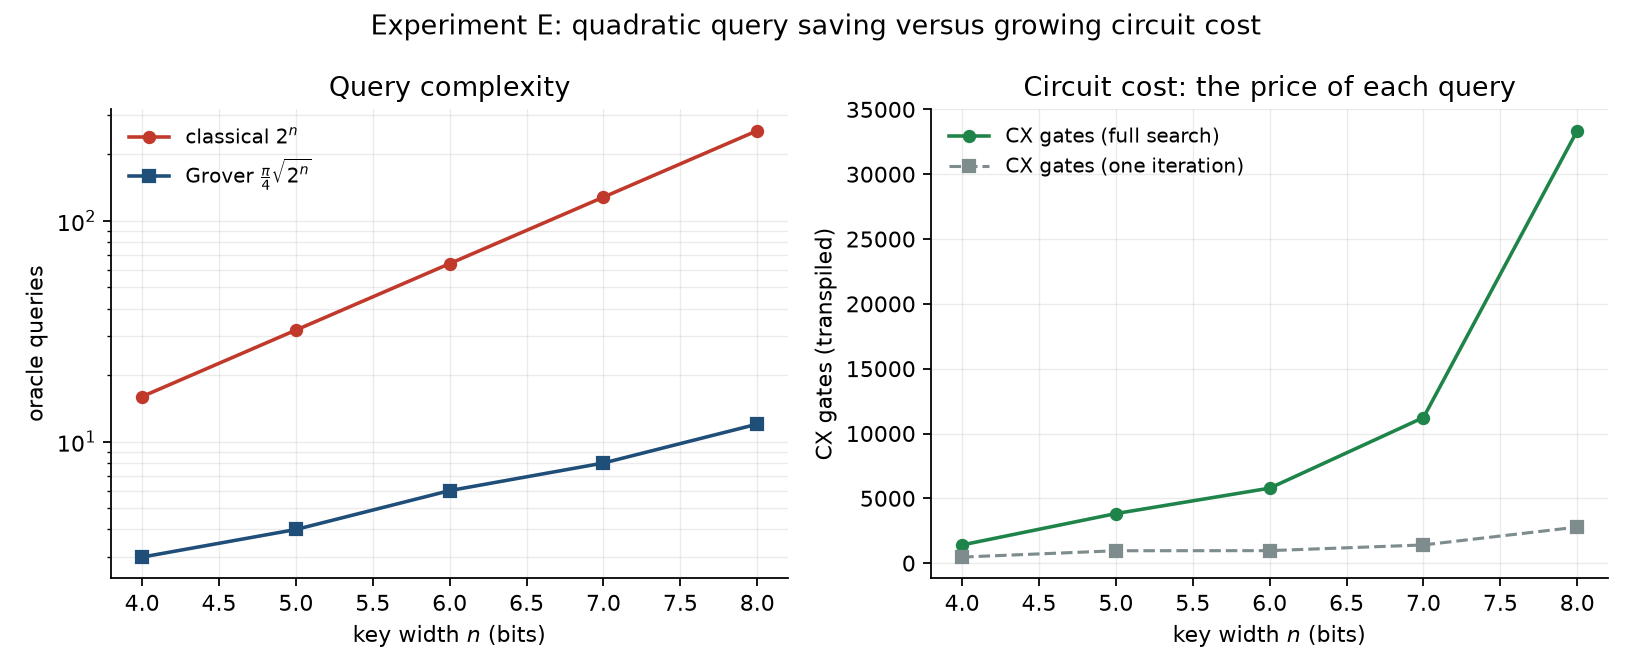
\includegraphics[width=0.98\textwidth]{fig6_resources.png}
  \caption{Experiment E. The quadratic query saving (left) set against the
    circuit cost of each query (right).}
  \label{fig:resources}
\end{figure}

The quadratic saving is real and visible in the $k^\ast$ column. But each query
costs a circuit, and the CX count rises from $\EminCx$ at $n=\EminKeyBits$ to
$\EmaxCx$ at $n=\EmaxKeyBits$ --- driven jointly by the cipher, the iteration
count, and the number of plaintext pairs required for a unique key
(Section~\ref{sec:pairs}).

The $\EmaxKeyBits$-bit configuration also illustrates
Section~\ref{sec:memory} concretely: at $\EmaxQubits$ qubits, density-matrix
simulation would need $\EmaxDensityGB$\,GB, whereas a trajectory statevector
needs $\EmaxStatevectorMB$\,MB. The memory barrier is removed; by
Eq.~\eqref{eq:runtime} the runtime cost remains, which is why these circuits are
counted rather than simulated.

This distinction --- between a query-complexity speedup and a resource estimate
--- is the connection to the AES literature~\citep{grassl2016,jaques2020}: the
query count is the easy part.

\paragraph{The speedup does not parallelise.} One further caveat belongs with any
statement of the quadratic saving, because it is what makes the saving far less
threatening in practice. Grover's algorithm \emph{cannot be parallelised better
than by partitioning the search space across independent quantum
computers}~\citep{zalka1999}. Splitting a search of size $N$ across $p$ machines
gives each a subspace of size $N/p$ and hence $\sqrt{N/p}$ queries, a saving of
only $\sqrt{p}$ rather than the factor $p$ that classical exhaustive search
enjoys. The $\Omega(\sqrt{N})$ lower bound~\citep{bennett1997,zalka1999} means no
better schedule exists.

The consequence is that the $k^\ast$ column of Table~\ref{tab:e} is essentially
a \emph{sequential depth}, not a cost that can be spent down with more hardware.
Combined with the CX counts beside it, this is why \citet{jaques2020} conclude
that Grover key search against AES remains out of reach even under generous
assumptions: the attack is depth-bound, and depth is precisely what a noisy
device cannot supply. Our Experiment~D threshold is the same conclusion in
miniature.

%==============================================================================
\section{Discussion}
%==============================================================================

Taken together the experiments give a consistent and unflattering picture of
Grover-based cryptanalysis on unmitigated NISQ hardware.

\paragraph{The algorithm is not the bottleneck.} Experiment A shows the oracle
and amplification are exact to floating-point precision. Nothing in the
algorithm limits the attack; what limits it is the physical cost of executing
$\Bcx$ two-qubit gates coherently.

\paragraph{Mitigation is channel-specific, and knowing which channel matters.}
The natural expectation is that error mitigation partially recovers a degraded
signal. Experiment C shows the truth is sharper and more useful: recovery is
near-total when the mitigated channel is the dominant one and exactly nil
otherwise. Reporting an average over both regimes would have obscured this.
The practical consequence is that one should characterise \emph{which} channel
dominates before selecting a mitigation strategy --- and for deep circuits the
answer will be gate error, for which zero-noise
extrapolation~\citep{temme2017,li2017} rather than readout inversion is the
appropriate tool.

\paragraph{Unphysical estimators are a real hazard.} That \texttt{pinv} reported
a success probability above the ideal value, with negative probability mass, is
worth emphasising because the failure is not loud. It produces a plausible
number that happens to be impossible. Constrained inversion should be the
default, and validity should be asserted rather than assumed.

\paragraph{Oracle design costs more than oracle queries.} The requirement for
multiple plaintext pairs (Section~\ref{sec:pairs}) emerged from measurement
rather than from design, and it multiplies both qubit count and circuit depth.
This mirrors the AES resource-estimation
literature~\citep{grassl2016,jaques2020}, where the reversible cipher
implementation, not the $2^{n/2}$ query count, dominates the cost.

\paragraph{Scope.} Grover is not the only quantum threat to symmetric
cryptography, and possibly not the most interesting one. Superposition attacks
based on Simon's algorithm give \emph{exponential} advantage against certain
constructions~\citep{kuwakado2010,kaplan2016}, a qualitatively different threat
model that the quadratic-speedup framing does not capture.

%==============================================================================
\section{Limitations}
\label{sec:limitations}
%==============================================================================

\begin{enumerate}
  \item \textbf{A 4-bit key is not cryptography.} It is a controlled testbed for
        oracle construction, amplification, noise and mitigation. Nothing here
        bears on the security of any deployed cipher.
  \item \textbf{Gate counts are upper bounds.} The S-box is exact but
        synthesised from its permutation matrix by quantum Shannon
        decomposition~\citep{shende2006}, costing roughly 95 CX. A
        hand-optimised Toffoli network~\citep{barenco1995,amy2016} would be
        substantially cheaper, so all reported counts are upper bounds rather
        than optimal estimates.
  \item \textbf{The noise model is a simplification.} Uniform depolarizing and
        readout error only, with no $T_1$/$T_2$ relaxation, crosstalk, leakage,
        parameter drift or correlated readout error. Real devices are both worse
        and less uniform.
  \item \textbf{Noiseless \texttt{rz} is an idealisation, and a load-bearing
        one.} Virtual Z gates have zero duration~\citep{mckay2017} and IBM
        reports no error for them, but the measured error is small rather than
        zero. Since \texttt{rz} is the most common gate after transpilation
        (roughly half of all gates), assigning it even $10^{-4}$ error would
        contribute comparably to the CX channel. Our noise estimates are
        therefore optimistic in this specific respect, which strengthens rather
        than weakens the negative result of Section~\ref{sec:results-c}.
  \item \textbf{Mitigation is not correction.} Post-processing a classical
        histogram corrects no quantum state; Experiment C measures precisely
        where that boundary lies.
  \item \textbf{Calibration is exponential} in the number of measured qubits
        ($2^{n}$ circuits). Tractable here only because the key register alone
        is measured; beyond roughly ten measured qubits a tensored or
        subspace-reduced method~\citep{nation2021} is required.
  \item \textbf{$M$ is obtained by classical brute force} in order to set
        $k^\ast$. This is legitimate for studying algorithmic behaviour, but a
        genuine attacker ignorant of $M$ would use the exponential-search
        schedule of~\citet{boyer1998}.
  \item \textbf{Energy claims are deliberately weak.} Trajectory sampling
        reduces memory from $4^n$ to $2^n$, and runtime maps loosely onto energy
        consumed~\citep{lannelongue2021}; reversible computation carries no
        thermodynamic lower bound per
        operation~\citep{landauer1961,bennett1973}. We make an algorithmic
        choice with a favourable scaling consequence and do not claim to have
        measured energy savings.
\end{enumerate}

%==============================================================================
\section{Conclusions and future work}
%==============================================================================

We built and exhaustively validated a reversible quantum oracle for
known-plaintext key search against a toy SPN, confirmed that Grover
amplification matches theory to $\AdeviationSci$, and showed that at
contemporary error rates the attack is not degraded but eliminated, with output
entropy $\Bentropy$ of $\BentropyMax$ bits. Classical readout-error mitigation
recovers a readout-limited signal almost completely
($\CReadoutRaw \to \CReadoutNnlsP$, ideal $\CidealP$) and a gate-error-limited
one not at all ($\CFullRaw \to \CFullNnlsP$). Recovery requires two-qubit error
rates at or below $\DmaxWorkingPtwo$, and the quadratic query saving is bought
with circuits growing to $\EmaxCx$ CX gates by $n = \EmaxKeyBits$.

Four extensions follow directly:

\begin{itemize}
  \item \textbf{Zero-noise extrapolation} for gate
        error~\citep{temme2017,li2017}. The noise-scaling machinery Experiment D
        already uses is exactly the mechanism ZNE requires.
  \item \textbf{Hand-optimised Toffoli S-box synthesis}, converting the resource
        counts from upper bounds into tight estimates and making deeper
        configurations simulable.
  \item \textbf{Scalable calibration}~\citep{nation2021} to pass the $2^n$
        calibration wall and reach wider key registers.
  \item \textbf{Superposition attacks} in the Simon's-algorithm
        family~\citep{kuwakado2010,kaplan2016}, which threaten certain symmetric
        constructions exponentially rather than quadratically.
\end{itemize}

\paragraph{Reproducibility.} All code, seeded configurations, raw JSON records
including full output distributions, and figure-generation scripts are released
with this report. Every number printed above is generated directly from the
saved records, so the report cannot drift from its data.

%==============================================================================
\bibliographystyle{plainnat}
\bibliography{references}
%==============================================================================

\end{document}
